%!TEX root=thesis.tex
\chapter{Appendix}

\section{Important Quantum Mechanics Concepts}

This section is meant to present a few fundamental ideas that are used throughout this work, but for a more thorough description of quantum mechanics see
\cite{mcintyre2012quantum, sakurai2017modern}.
In all equations that follow, $\hbar = 1$ is assumed.

% state of system <-> density operator
Given a quantum system, a general state can be represented by a density operator $\rho(t)$. The density operator encapsulates all known information about the quantum system, specifically the expectation values associated with well-defined observable.
The density operator is Hermitian ($\rho^\dagger = \rho$) and $\Tr(\rho) = 1$.
For an observable $\hat{A}$, there is a corresponding Hermitian operator $A$, with the expectation is given by
\begin{equation}\label{eq:measure}
    \langle A \rangle = \Tr{\rho A}
\end{equation}

The time evolution of the density operator is given by
\begin{equation}\label{eq:density-time}
    \rho(t) = U(t) \rho(0) U(t)^\dagger
\end{equation}
where the unitary operator $U$ is the ``propagator'' defined by
\begin{equation}\label{eq:propagator-de}
    i \ddt{U(t)} = H(t) U(t), U(0) = \identity
\end{equation}
% The two equations above can be combined to yield the Liouville-Von Neumann equation, which explicitly shows the density operator's time evolution from the system Hamiltonian.
% \begin{equation}
%     i \ddt{\rho(t)} = [H(t), \rho(t)]
% \end{equation}

When the Hamiltonian is time-independent or if the Hamiltonian commutes with itself at different points in time (i.e. $[H(t_1), H(t_2)] = 0$), equation~\ref{eq:propagator-de} can be solved to obtain the propagator
\begin{equation}\label{eq:propagator-ti}
    U(t) = \text{exp}\left[ {-i \int_0^t H(t') dt'} \right]
\end{equation}
However, if the Hamiltonian is time-dependent and doesn't commute with itself at different times, then the above equation is not valid. This difficulty with time-dependent Hamiltonians and methods with dealing with them are further discussed in~\ref{sec:AHT}.

In many cases it can be helpful to consider the \emph{interaction frame} of a particular interaction. If the Hamiltonian is expressed as the sum of two terms
\[
H(t) = H_A(t) + H_B(t)
\]
then there is a unitary operator $U_A(t)$ given by
\begin{equation}\label{eq:interaction-propagator}
    \frac{d}{dt} U_A(t) = -i H_A(t) U_A(t), \, U_A(0) = \identity
\end{equation}
that maps from the interaction frame to the lab frame.
The dynamics in the interaction frame are described by the interaction frame Hamiltonian $\widetilde{H}(t) = {U_A(t)}^{\dagger} H_B(t)U_A(t)$
\[
\frac{d}{dt}\widetilde{U}(t) = -i \widetilde{H}(t)\widetilde{U}(t),\, \widetilde{U}(0) = \identity
\]
The propagator in the lab frame $U(t)$ is related to $\widetilde{U}(t)$ by first time evolution in the interaction frame, then mapping from the interaction frame to the lab frame
\[
U(t) = U_A(t)\widetilde{U}(t).
\]

\section{Neural Network Architecture}

\begin{figure}[H]
    \centering
    

\tikzset{every picture/.style={line width=0.75pt}} %set default line width to 0.75pt

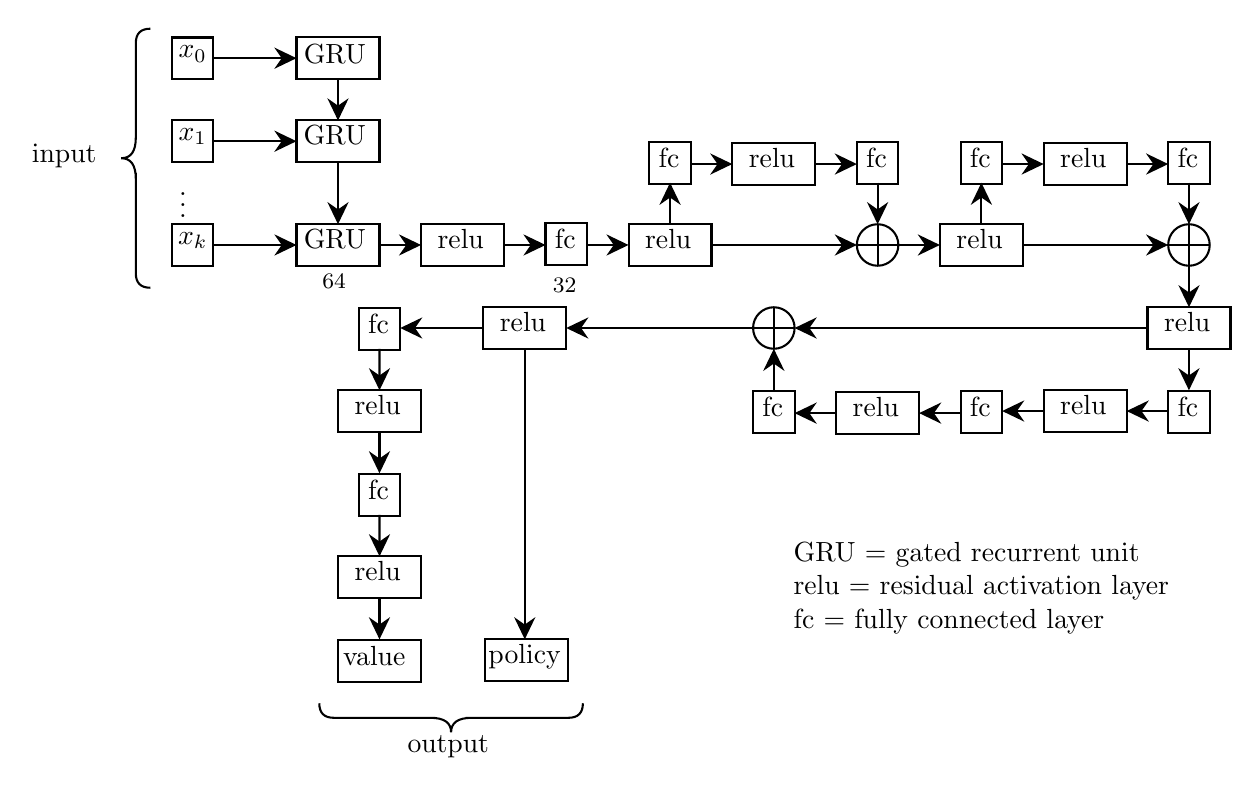
\begin{tikzpicture}[x=0.75pt,y=0.75pt,yscale=-1,xscale=1]
%uncomment if require: \path (0,382); %set diagram left start at 0, and has height of 382

%Shape: Rectangle [id:dp02638136849538708]
\draw   (90.01,20.25) -- (110.01,20.25) -- (110.01,40.25) -- (90.01,40.25) -- cycle ;
%Shape: Rectangle [id:dp4204285901048066]
\draw   (90,60.2) -- (110,60.2) -- (110,80.2) -- (90,80.2) -- cycle ;
%Straight Lines [id:da18786128196874485]
\draw    (110.02,30.2) -- (147.02,30.2) ;
\draw [shift={(150.02,30.2)}, rotate = 180] [fill={rgb, 255:red, 0; green, 0; blue, 0 }  ][line width=0.08]  [draw opacity=0] (10.72,-5.15) -- (0,0) -- (10.72,5.15) -- (7.12,0) -- cycle    ;
%Straight Lines [id:da8836932503131412]
\draw    (110.01,70.2) -- (147.01,70.2) ;
\draw [shift={(150.01,70.2)}, rotate = 180] [fill={rgb, 255:red, 0; green, 0; blue, 0 }  ][line width=0.08]  [draw opacity=0] (10.72,-5.15) -- (0,0) -- (10.72,5.15) -- (7.12,0) -- cycle    ;
%Straight Lines [id:da3922749523317497]
\draw    (170.02,40.2) -- (170.02,57.2) ;
\draw [shift={(170.02,60.2)}, rotate = 270] [fill={rgb, 255:red, 0; green, 0; blue, 0 }  ][line width=0.08]  [draw opacity=0] (10.72,-5.15) -- (0,0) -- (10.72,5.15) -- (7.12,0) -- cycle    ;
%Shape: Rectangle [id:dp32409815423962685]
\draw   (150.02,20.2) -- (190.02,20.2) -- (190.02,40.2) -- (150.02,40.2) -- cycle ;
%Shape: Rectangle [id:dp7239061253067598]
\draw   (150.01,60.2) -- (190.01,60.2) -- (190.01,80.2) -- (150.01,80.2) -- cycle ;
%Shape: Rectangle [id:dp7205034746760461]
\draw   (90.01,110.2) -- (110.01,110.2) -- (110.01,130.2) -- (90.01,130.2) -- cycle ;
%Straight Lines [id:da2768291231406834]
\draw    (110.02,120.2) -- (147.02,120.2) ;
\draw [shift={(150.02,120.2)}, rotate = 180] [fill={rgb, 255:red, 0; green, 0; blue, 0 }  ][line width=0.08]  [draw opacity=0] (10.72,-5.15) -- (0,0) -- (10.72,5.15) -- (7.12,0) -- cycle    ;
%Straight Lines [id:da04420279990164899]
\draw    (170.02,80.2) -- (170.02,107.2) ;
\draw [shift={(170.02,110.2)}, rotate = 270] [fill={rgb, 255:red, 0; green, 0; blue, 0 }  ][line width=0.08]  [draw opacity=0] (10.72,-5.15) -- (0,0) -- (10.72,5.15) -- (7.12,0) -- cycle    ;
%Shape: Rectangle [id:dp5376553256891963]
\draw   (150.02,110.2) -- (190.02,110.2) -- (190.02,130.2) -- (150.02,130.2) -- cycle ;
%Shape: Rectangle [id:dp20156185382495795]
\draw   (210.02,110.2) -- (250,110.2) -- (250,130.2) -- (210.02,130.2) -- cycle ;
%Straight Lines [id:da792263985693916]
\draw    (190.02,120.2) -- (207.02,120.2) ;
\draw [shift={(210.02,120.2)}, rotate = 180] [fill={rgb, 255:red, 0; green, 0; blue, 0 }  ][line width=0.08]  [draw opacity=0] (10.72,-5.15) -- (0,0) -- (10.72,5.15) -- (7.12,0) -- cycle    ;
%Straight Lines [id:da6470713620273096]
\draw    (430,90.2) -- (430,107.2) ;
\draw [shift={(430,110.2)}, rotate = 270] [fill={rgb, 255:red, 0; green, 0; blue, 0 }  ][line width=0.08]  [draw opacity=0] (10.72,-5.15) -- (0,0) -- (10.72,5.15) -- (7.12,0) -- cycle    ;
%Flowchart: Or [id:dp6599768898399976]
\draw   (420,120.2) .. controls (420,114.68) and (424.48,110.2) .. (430,110.2) .. controls (435.52,110.2) and (440,114.68) .. (440,120.2) .. controls (440,125.72) and (435.52,130.2) .. (430,130.2) .. controls (424.48,130.2) and (420,125.72) .. (420,120.2) -- cycle ; \draw   (420,120.2) -- (440,120.2) ; \draw   (430,110.2) -- (430,130.2) ;
%Shape: Rectangle [id:dp7585346138321025]
\draw   (270,109.7) -- (290,109.7) -- (290,129.7) -- (270,129.7) -- cycle ;
%Straight Lines [id:da5278108394530496]
\draw    (250,120.2) -- (267,120.2) ;
\draw [shift={(270,120.2)}, rotate = 180] [fill={rgb, 255:red, 0; green, 0; blue, 0 }  ][line width=0.08]  [draw opacity=0] (10.72,-5.15) -- (0,0) -- (10.72,5.15) -- (7.12,0) -- cycle    ;
%Shape: Rectangle [id:dp45637585865043273]
\draw   (310,110.2) -- (349.98,110.2) -- (349.98,130.2) -- (310,130.2) -- cycle ;
%Straight Lines [id:da015144151772794379]
\draw    (290,120.2) -- (307,120.2) ;
\draw [shift={(310,120.2)}, rotate = 180] [fill={rgb, 255:red, 0; green, 0; blue, 0 }  ][line width=0.08]  [draw opacity=0] (10.72,-5.15) -- (0,0) -- (10.72,5.15) -- (7.12,0) -- cycle    ;
%Shape: Rectangle [id:dp680216878775233]
\draw   (320,70.7) -- (340,70.7) -- (340,90.7) -- (320,90.7) -- cycle ;
%Shape: Rectangle [id:dp7310722650845467]
\draw   (360,71.2) -- (399.98,71.2) -- (399.98,91.2) -- (360,91.2) -- cycle ;
%Straight Lines [id:da476677827076349]
\draw    (340,81.2) -- (357,81.2) ;
\draw [shift={(360,81.2)}, rotate = 180] [fill={rgb, 255:red, 0; green, 0; blue, 0 }  ][line width=0.08]  [draw opacity=0] (10.72,-5.15) -- (0,0) -- (10.72,5.15) -- (7.12,0) -- cycle    ;
%Straight Lines [id:da9800517663487802]
\draw    (330,110.2) -- (330,93.2) ;
\draw [shift={(330,90.2)}, rotate = 450] [fill={rgb, 255:red, 0; green, 0; blue, 0 }  ][line width=0.08]  [draw opacity=0] (10.72,-5.15) -- (0,0) -- (10.72,5.15) -- (7.12,0) -- cycle    ;
%Shape: Rectangle [id:dp021057905114674424]
\draw   (420,70.7) -- (440,70.7) -- (440,90.7) -- (420,90.7) -- cycle ;
%Straight Lines [id:da19829953520297927]
\draw    (400,81.2) -- (417,81.2) ;
\draw [shift={(420,81.2)}, rotate = 180] [fill={rgb, 255:red, 0; green, 0; blue, 0 }  ][line width=0.08]  [draw opacity=0] (10.72,-5.15) -- (0,0) -- (10.72,5.15) -- (7.12,0) -- cycle    ;
%Straight Lines [id:da37662612388777994]
\draw    (350,120.2) -- (417,120.2) ;
\draw [shift={(420,120.2)}, rotate = 180] [fill={rgb, 255:red, 0; green, 0; blue, 0 }  ][line width=0.08]  [draw opacity=0] (10.72,-5.15) -- (0,0) -- (10.72,5.15) -- (7.12,0) -- cycle    ;
%Shape: Rectangle [id:dp5579644555480454]
\draw   (560.02,150.2) -- (600,150.2) -- (600,170.2) -- (560.02,170.2) -- cycle ;
%Straight Lines [id:da06494630042228744]
\draw    (580.02,130.2) -- (580.02,147.2) ;
\draw [shift={(580.02,150.2)}, rotate = 270] [fill={rgb, 255:red, 0; green, 0; blue, 0 }  ][line width=0.08]  [draw opacity=0] (10.72,-5.15) -- (0,0) -- (10.72,5.15) -- (7.12,0) -- cycle    ;
%Straight Lines [id:da8876672874205853]
\draw    (580,90.2) -- (580,107.2) ;
\draw [shift={(580,110.2)}, rotate = 270] [fill={rgb, 255:red, 0; green, 0; blue, 0 }  ][line width=0.08]  [draw opacity=0] (10.72,-5.15) -- (0,0) -- (10.72,5.15) -- (7.12,0) -- cycle    ;
%Flowchart: Or [id:dp7508932175580134]
\draw   (570,120.2) .. controls (570,114.68) and (574.48,110.2) .. (580,110.2) .. controls (585.52,110.2) and (590,114.68) .. (590,120.2) .. controls (590,125.72) and (585.52,130.2) .. (580,130.2) .. controls (574.48,130.2) and (570,125.72) .. (570,120.2) -- cycle ; \draw   (570,120.2) -- (590,120.2) ; \draw   (580,110.2) -- (580,130.2) ;
%Shape: Rectangle [id:dp49517683581388927]
\draw   (460,110.2) -- (499.98,110.2) -- (499.98,130.2) -- (460,130.2) -- cycle ;
%Straight Lines [id:da9885418731285747]
\draw    (440,120.2) -- (457,120.2) ;
\draw [shift={(460,120.2)}, rotate = 180] [fill={rgb, 255:red, 0; green, 0; blue, 0 }  ][line width=0.08]  [draw opacity=0] (10.72,-5.15) -- (0,0) -- (10.72,5.15) -- (7.12,0) -- cycle    ;
%Shape: Rectangle [id:dp7101148618833939]
\draw   (470,70.7) -- (490,70.7) -- (490,90.7) -- (470,90.7) -- cycle ;
%Shape: Rectangle [id:dp6761712905766428]
\draw   (510,71.2) -- (549.98,71.2) -- (549.98,91.2) -- (510,91.2) -- cycle ;
%Straight Lines [id:da7602138343769007]
\draw    (490,81.2) -- (507,81.2) ;
\draw [shift={(510,81.2)}, rotate = 180] [fill={rgb, 255:red, 0; green, 0; blue, 0 }  ][line width=0.08]  [draw opacity=0] (10.72,-5.15) -- (0,0) -- (10.72,5.15) -- (7.12,0) -- cycle    ;
%Straight Lines [id:da44997478868284935]
\draw    (480,110.2) -- (480,93.2) ;
\draw [shift={(480,90.2)}, rotate = 450] [fill={rgb, 255:red, 0; green, 0; blue, 0 }  ][line width=0.08]  [draw opacity=0] (10.72,-5.15) -- (0,0) -- (10.72,5.15) -- (7.12,0) -- cycle    ;
%Shape: Rectangle [id:dp8001219618459012]
\draw   (570,70.7) -- (590,70.7) -- (590,90.7) -- (570,90.7) -- cycle ;
%Straight Lines [id:da8191439427145315]
\draw    (550,81.2) -- (567,81.2) ;
\draw [shift={(570,81.2)}, rotate = 180] [fill={rgb, 255:red, 0; green, 0; blue, 0 }  ][line width=0.08]  [draw opacity=0] (10.72,-5.15) -- (0,0) -- (10.72,5.15) -- (7.12,0) -- cycle    ;
%Straight Lines [id:da9263282941037065]
\draw    (500,120.2) -- (567,120.2) ;
\draw [shift={(570,120.2)}, rotate = 180] [fill={rgb, 255:red, 0; green, 0; blue, 0 }  ][line width=0.08]  [draw opacity=0] (10.72,-5.15) -- (0,0) -- (10.72,5.15) -- (7.12,0) -- cycle    ;
%Straight Lines [id:da1317984498790985]
\draw    (580,170.2) -- (580,187.2) ;
\draw [shift={(580,190.2)}, rotate = 270] [fill={rgb, 255:red, 0; green, 0; blue, 0 }  ][line width=0.08]  [draw opacity=0] (10.72,-5.15) -- (0,0) -- (10.72,5.15) -- (7.12,0) -- cycle    ;
%Shape: Rectangle [id:dp19231745792682342]
\draw   (570,190.7) -- (590,190.7) -- (590,210.7) -- (570,210.7) -- cycle ;
%Shape: Rectangle [id:dp3661262539844976]
\draw   (510,190.2) -- (549.98,190.2) -- (549.98,210.2) -- (510,210.2) -- cycle ;
%Straight Lines [id:da46430121112477796]
\draw    (570,200.2) -- (553,200.2) ;
\draw [shift={(550,200.2)}, rotate = 360] [fill={rgb, 255:red, 0; green, 0; blue, 0 }  ][line width=0.08]  [draw opacity=0] (10.72,-5.15) -- (0,0) -- (10.72,5.15) -- (7.12,0) -- cycle    ;
%Shape: Rectangle [id:dp7015582656278725]
\draw   (470,190.7) -- (490,190.7) -- (490,210.7) -- (470,210.7) -- cycle ;
%Straight Lines [id:da6274160240081927]
\draw    (510,200.2) -- (493,200.2) ;
\draw [shift={(490,200.2)}, rotate = 360] [fill={rgb, 255:red, 0; green, 0; blue, 0 }  ][line width=0.08]  [draw opacity=0] (10.72,-5.15) -- (0,0) -- (10.72,5.15) -- (7.12,0) -- cycle    ;
%Shape: Rectangle [id:dp5757706276069112]
\draw   (410,191.2) -- (449.98,191.2) -- (449.98,211.2) -- (410,211.2) -- cycle ;
%Straight Lines [id:da877816695924893]
\draw    (470,201.2) -- (453,201.2) ;
\draw [shift={(450,201.2)}, rotate = 360] [fill={rgb, 255:red, 0; green, 0; blue, 0 }  ][line width=0.08]  [draw opacity=0] (10.72,-5.15) -- (0,0) -- (10.72,5.15) -- (7.12,0) -- cycle    ;
%Shape: Rectangle [id:dp9665386619854055]
\draw   (370,190.7) -- (390,190.7) -- (390,210.7) -- (370,210.7) -- cycle ;
%Straight Lines [id:da43350283631446174]
\draw    (410,201.2) -- (393,201.2) ;
\draw [shift={(390,201.2)}, rotate = 360] [fill={rgb, 255:red, 0; green, 0; blue, 0 }  ][line width=0.08]  [draw opacity=0] (10.72,-5.15) -- (0,0) -- (10.72,5.15) -- (7.12,0) -- cycle    ;
%Flowchart: Or [id:dp6555350236573219]
\draw   (370,160.2) .. controls (370,154.68) and (374.48,150.2) .. (380,150.2) .. controls (385.52,150.2) and (390,154.68) .. (390,160.2) .. controls (390,165.72) and (385.52,170.2) .. (380,170.2) .. controls (374.48,170.2) and (370,165.72) .. (370,160.2) -- cycle ; \draw   (370,160.2) -- (390,160.2) ; \draw   (380,150.2) -- (380,170.2) ;
%Straight Lines [id:da9538541164521721]
\draw    (560,160.2) -- (393,160.2) ;
\draw [shift={(390,160.2)}, rotate = 360] [fill={rgb, 255:red, 0; green, 0; blue, 0 }  ][line width=0.08]  [draw opacity=0] (10.72,-5.15) -- (0,0) -- (10.72,5.15) -- (7.12,0) -- cycle    ;
%Straight Lines [id:da10469597971614442]
\draw    (380,190.2) -- (380,173.2) ;
\draw [shift={(380,170.2)}, rotate = 450] [fill={rgb, 255:red, 0; green, 0; blue, 0 }  ][line width=0.08]  [draw opacity=0] (10.72,-5.15) -- (0,0) -- (10.72,5.15) -- (7.12,0) -- cycle    ;
%Shape: Rectangle [id:dp07415870480577125]
\draw   (240.02,150.2) -- (280,150.2) -- (280,170.2) -- (240.02,170.2) -- cycle ;
%Straight Lines [id:da857184847829574]
\draw    (370,160.2) -- (283,160.2) ;
\draw [shift={(280,160.2)}, rotate = 360] [fill={rgb, 255:red, 0; green, 0; blue, 0 }  ][line width=0.08]  [draw opacity=0] (10.72,-5.15) -- (0,0) -- (10.72,5.15) -- (7.12,0) -- cycle    ;
%Shape: Rectangle [id:dp7255363648906021]
\draw   (241.01,310.2) -- (280.99,310.2) -- (280.99,330.2) -- (241.01,330.2) -- cycle ;
%Straight Lines [id:da10818889394863507]
\draw    (260,170.2) -- (260,307.2) ;
\draw [shift={(260,310.2)}, rotate = 270] [fill={rgb, 255:red, 0; green, 0; blue, 0 }  ][line width=0.08]  [draw opacity=0] (10.72,-5.15) -- (0,0) -- (10.72,5.15) -- (7.12,0) -- cycle    ;
%Shape: Rectangle [id:dp8701695128090077]
\draw   (180,150.7) -- (200,150.7) -- (200,170.7) -- (180,170.7) -- cycle ;
%Straight Lines [id:da0015163063151002465]
\draw    (240,160.2) -- (203,160.2) ;
\draw [shift={(200,160.2)}, rotate = 360] [fill={rgb, 255:red, 0; green, 0; blue, 0 }  ][line width=0.08]  [draw opacity=0] (10.72,-5.15) -- (0,0) -- (10.72,5.15) -- (7.12,0) -- cycle    ;
%Shape: Rectangle [id:dp11711776574433075]
\draw   (170.02,190.2) -- (210,190.2) -- (210,210.2) -- (170.02,210.2) -- cycle ;
%Straight Lines [id:da909719887882497]
\draw    (190,170.2) -- (190.02,187.2) ;
\draw [shift={(190.02,190.2)}, rotate = 269.93] [fill={rgb, 255:red, 0; green, 0; blue, 0 }  ][line width=0.08]  [draw opacity=0] (10.72,-5.15) -- (0,0) -- (10.72,5.15) -- (7.12,0) -- cycle    ;
%Straight Lines [id:da057281968974082886]
\draw    (190,210.2) -- (190,227.2) ;
\draw [shift={(190,230.2)}, rotate = 270] [fill={rgb, 255:red, 0; green, 0; blue, 0 }  ][line width=0.08]  [draw opacity=0] (10.72,-5.15) -- (0,0) -- (10.72,5.15) -- (7.12,0) -- cycle    ;
%Shape: Rectangle [id:dp11366092940797157]
\draw   (180,230.7) -- (200,230.7) -- (200,250.7) -- (180,250.7) -- cycle ;
%Shape: Rectangle [id:dp7686918520673491]
\draw   (170.02,270.2) -- (210,270.2) -- (210,290.2) -- (170.02,290.2) -- cycle ;
%Straight Lines [id:da284359228138074]
\draw    (190,250.2) -- (190.02,267.2) ;
\draw [shift={(190.02,270.2)}, rotate = 269.93] [fill={rgb, 255:red, 0; green, 0; blue, 0 }  ][line width=0.08]  [draw opacity=0] (10.72,-5.15) -- (0,0) -- (10.72,5.15) -- (7.12,0) -- cycle    ;
%Straight Lines [id:da5969772278968581]
\draw    (190,290.2) -- (190,307.2) ;
\draw [shift={(190,310.2)}, rotate = 270] [fill={rgb, 255:red, 0; green, 0; blue, 0 }  ][line width=0.08]  [draw opacity=0] (10.72,-5.15) -- (0,0) -- (10.72,5.15) -- (7.12,0) -- cycle    ;
%Shape: Rectangle [id:dp6607557330878455]
\draw   (170,310.7) -- (210,310.7) -- (210,330.7) -- (170,330.7) -- cycle ;
%Shape: Brace [id:dp14557160899369648]
\draw   (79.6,16) .. controls (74.93,16) and (72.6,18.33) .. (72.6,23) -- (72.6,68.4) .. controls (72.6,75.07) and (70.27,78.4) .. (65.6,78.4) .. controls (70.27,78.4) and (72.6,81.73) .. (72.6,88.4)(72.6,85.4) -- (72.6,133.8) .. controls (72.6,138.47) and (74.93,140.8) .. (79.6,140.8) ;
%Shape: Brace [id:dp11478022100821583]
\draw   (161,341) .. controls (161,345.67) and (163.33,348) .. (168,348) -- (214.5,348) .. controls (221.17,348) and (224.5,350.33) .. (224.5,355) .. controls (224.5,350.33) and (227.83,348) .. (234.5,348)(231.5,348) -- (281,348) .. controls (285.67,348) and (288,345.67) .. (288,341) ;

% Text Node
\draw (100.02,28.2) node    {$x_{0}$};
% Text Node
\draw (100.01,68.15) node    {$x_{1}$};
% Text Node
\draw (152.02,22.2) node [anchor=north west][inner sep=0.75pt]   [align=left] {GRU};
% Text Node
\draw (152.01,61.2) node [anchor=north west][inner sep=0.75pt]   [align=left] {GRU};
% Text Node
\draw (92.01,85.6) node [anchor=north west][inner sep=0.75pt]    {$\vdots $};
% Text Node
\draw (100.02,118.15) node    {$x_{k}$};
% Text Node
\draw (152.02,111.2) node [anchor=north west][inner sep=0.75pt]   [align=left] {GRU};
% Text Node
\draw (216.51,111.2) node [anchor=north west][inner sep=0.75pt]   [align=left] {relu};
% Text Node
\draw (161.02,132.6) node [anchor=north west][inner sep=0.75pt]  [font=\footnotesize]  {$64$};
% Text Node
\draw (272,134.6) node [anchor=north west][inner sep=0.75pt]  [font=\footnotesize]  {$32$};
% Text Node
\draw (273,111.2) node [anchor=north west][inner sep=0.75pt]   [align=left] {fc};
% Text Node
\draw (316.49,111.2) node [anchor=north west][inner sep=0.75pt]   [align=left] {relu};
% Text Node
\draw (323,72.2) node [anchor=north west][inner sep=0.75pt]   [align=left] {fc};
% Text Node
\draw (366.49,72.2) node [anchor=north west][inner sep=0.75pt]   [align=left] {relu};
% Text Node
\draw (423,72.2) node [anchor=north west][inner sep=0.75pt]   [align=left] {fc};
% Text Node
\draw (566.51,151.2) node [anchor=north west][inner sep=0.75pt]   [align=left] {relu};
% Text Node
\draw (466.49,111.2) node [anchor=north west][inner sep=0.75pt]   [align=left] {relu};
% Text Node
\draw (473,72.2) node [anchor=north west][inner sep=0.75pt]   [align=left] {fc};
% Text Node
\draw (516.49,72.2) node [anchor=north west][inner sep=0.75pt]   [align=left] {relu};
% Text Node
\draw (573,72.2) node [anchor=north west][inner sep=0.75pt]   [align=left] {fc};
% Text Node
\draw (573,192.2) node [anchor=north west][inner sep=0.75pt]   [align=left] {fc};
% Text Node
\draw (516.49,191.2) node [anchor=north west][inner sep=0.75pt]   [align=left] {relu};
% Text Node
\draw (473,192.2) node [anchor=north west][inner sep=0.75pt]   [align=left] {fc};
% Text Node
\draw (416.49,192.2) node [anchor=north west][inner sep=0.75pt]   [align=left] {relu};
% Text Node
\draw (373,192.2) node [anchor=north west][inner sep=0.75pt]   [align=left] {fc};
% Text Node
\draw (246.51,151.2) node [anchor=north west][inner sep=0.75pt]   [align=left] {relu};
% Text Node
\draw (241,311.2) node [anchor=north west][inner sep=0.75pt]   [align=left] {policy};
% Text Node
\draw (183,152.2) node [anchor=north west][inner sep=0.75pt]   [align=left] {fc};
% Text Node
\draw (176.51,191.2) node [anchor=north west][inner sep=0.75pt]   [align=left] {relu};
% Text Node
\draw (183,232.2) node [anchor=north west][inner sep=0.75pt]   [align=left] {fc};
% Text Node
\draw (176.51,271.2) node [anchor=north west][inner sep=0.75pt]   [align=left] {relu};
% Text Node
\draw (171,312.2) node [anchor=north west][inner sep=0.75pt]   [align=left] {value};
% Text Node
\draw (21,70) node [anchor=north west][inner sep=0.75pt]   [align=left] {input};
% Text Node
\draw (202,355) node [anchor=north west][inner sep=0.75pt]   [align=left] {output};
% Text Node
\draw (388,262) node [anchor=north west][inner sep=0.75pt]   [align=left] {GRU = gated recurrent unit\\relu = residual activation layer\\fc = fully connected layer};


\end{tikzpicture}

    % \includegraphics{example-image}
    \caption{The policy and value network architecture.}
    \label{fig:nn}
\end{figure}
% TODO redo to have it go in straight line???

\section{Pulse Sequence Definitions}

\subsection{CORY48}


\begin{equation*}
\begin{aligned}
    X, \tau, Y, 2\tau, \overline{X}, \tau, Y, 2\tau, X, \tau, Y, 2\tau,
    X, \tau, Y, 2\tau, X, \tau, \overline{Y}, 2\tau, X, \tau, Y, 2\tau, \\
    %
    \overline{Y}, \tau, \overline{X}, 2\tau, Y, \tau, \overline{X}, 2\tau,
    \overline{Y}, \tau, \overline{X}, 2\tau, \overline{Y}, \tau, \overline{X},
    2\tau, \overline{Y}, \tau, X, 2\tau, \overline{Y}, \tau, \overline{X},
    2\tau, \\
    %
    \overline{X}, \tau, Y, 2\tau, \overline{X}, \tau, \overline{Y}, 2\tau,
    \overline{X}, \tau, Y, 2\tau, X, \tau, \overline{Y}, 2\tau, \overline{X},
    \tau, \overline{Y}, 2\tau, X, \tau, \overline{Y}, 2\tau, \\
    %
    Y, \tau, \overline{X}, 2\tau, Y, \tau, X, 2\tau, Y, \tau, \overline{X}, 2\tau, \overline{Y}, \tau, X, 2\tau, Y, \tau, X, 2\tau, \overline{Y}, \tau, X, 2\tau
\end{aligned}
\end{equation*}

\subsection{AlphaZero Pulse Sequences: No Errors}

\noindent $12\tau$

\begin{equation*}
\begin{aligned}
    X, \tau, \overline{Y}, \tau, \overline{Y}, \tau, X, \tau, \overline{Y}, \tau, \overline{Y}, \tau, \overline{Y}, \tau, X, \tau, X, \tau, \overline{Y}, \tau, X, \tau, X, \tau
\end{aligned}
\end{equation*}

\noindent $24\tau$

\begin{equation*}
\begin{aligned}
    \overline{Y}, \tau, \overline{Y}, \tau, \overline{X}, \tau, \overline{Y}, \tau, \overline{Y}, \tau, \overline{X}, \tau, \overline{Y}, \tau, \overline{Y}, \tau, X, \tau, X, \tau, \overline{Y}, \tau, X, \tau, \\
    \overline{Y}, \tau, \overline{Y}, \tau, X, \tau, \overline{Y}, \tau, \overline{Y}, \tau, X, \tau, X, \tau, X, \tau, \overline{Y}, \tau, \overline{Y}, \tau, X, \tau, \overline{Y}, \tau
\end{aligned}
\end{equation*}

\noindent $48\tau$

\begin{equation*}
\begin{aligned}
    \overline{Y}, \tau, \overline{X}, \tau, \overline{Y}, \tau, \overline{X}, \tau, \overline{Y}, \tau, \overline{X}, \tau, Y, \tau, X, \tau, Y, \tau, X, \tau, X, \tau, Y, \tau, \\
    Y, \tau, X, \tau, X, \tau, Y, \tau, X, \tau, X, 2\tau, \overline{X}, \tau, \overline{Y}, \tau, \overline{X}, \tau, \overline{X}, \tau, \overline{Y}, \tau, \overline{X}, \tau, \\
    \overline{X}, \tau, \overline{Y}, \tau, \overline{X}, \tau, \overline{Y}, \tau, \overline{X}, \tau, \overline{Y}, \tau, \overline{Y}, \tau,
    \overline{X}, \tau, \overline{X}, \tau, \overline{X}, \tau, \overline{Y}, 2\tau, \overline{Y}, \tau, \\
    \overline{Y}, \tau, \overline{X}, \tau, \overline{Y}, \tau, \overline{Y}, \tau, X, \tau, Y, \tau, \overline{X}, \tau, Y, \tau, \overline{X}, \tau, Y, \tau
\end{aligned}
\end{equation*}


\subsection{AlphaZero Pulse Sequences: Rotation Errors}

\noindent $12\tau$

\begin{equation*}
\begin{aligned}
    \tau, X, \tau, X, \tau, Y, \tau, X, \tau, X, 2\tau, \overline{X}, \tau, \overline{X}, \tau, \overline{Y}, \tau, \overline{X}, \tau, \overline{X}, \tau
\end{aligned}
\end{equation*}

\noindent $24\tau$

\begin{equation*}
\begin{aligned}
    \overline{Y}, \tau, X, \tau, Y, \tau, Y, \tau, X, \tau, Y, \tau, Y, \tau, \overline{X}, \tau, Y, \tau, Y, \tau, \overline{X}, \tau, Y, \tau, \\
    Y, \tau, \overline{X}, \tau, \overline{Y}, \tau, \overline{Y}, \tau, \overline{X}, \tau, \overline{Y}, \tau, \overline{Y}, \tau, X, \tau, \overline{Y}, \tau, \overline{Y}, \tau, X, \tau, \overline{Y}, \tau
\end{aligned}
\end{equation*}

\noindent $48\tau$

\begin{equation*}
\begin{aligned}
    \overline{Y}, \tau, \overline{Y}, \tau, \overline{X}, \tau, \overline{X}, \tau, \overline{X}, \tau, \overline{Y}, \tau, \overline{X}, \tau, Y, \tau, \overline{X}, \tau, \overline{X}, \tau, Y, \tau, \overline{X}, \tau, \\
    %
    \overline{Y}, \tau, \overline{X}, \tau, \overline{Y}, \tau, \overline{X}, \tau, \overline{X}, \tau, \overline{Y}, \tau, Y, \tau, \overline{X}, \tau,
    \overline{Y}, \tau, \overline{Y}, \tau, \overline{X}, \tau, \overline{Y}, \tau, \\
    %
    \overline{Y}, \tau, X, \tau, Y, \tau, Y, \tau, X, \tau, Y, \tau, Y, \tau, \overline{X}, \tau, \overline{X}, \tau, Y, \tau, \overline{X}, \tau, \overline{X}, \tau, \\
    %
    \overline{Y}, \tau, \overline{X}, \tau, \overline{X}, \tau, \overline{Y}, \tau, \overline{X}, \tau, \overline{X}, \tau, \overline{Y}, \tau,
    \overline{X}, \tau, \overline{X}, \tau, \overline{Y}, \tau, \overline{X}, \tau, \overline{X}, \tau
    %
\end{aligned}
\end{equation*}



\subsection{AlphaZero Pulse Sequences: All Errors}

\noindent $12\tau$

\begin{equation*}
\begin{aligned}
    \overline{Y}, \tau, \overline{X}, \tau, Y, \tau, Y, \tau, \overline{X}, \tau, Y, \tau, Y, \tau, \overline{X}, \tau, \overline{Y}, \tau, \overline{Y}, \tau, \overline{X}, \tau, \overline{Y}, \tau
\end{aligned}
\end{equation*}

\noindent $24\tau$

\begin{equation*}
\begin{aligned}
    \overline{Y}, \tau, \overline{Y}, \tau, \overline{X}, \tau, \overline{Y}, \tau, \overline{Y}, \tau, \overline{X}, \tau, Y, \tau, \overline{X}, \tau, Y, \tau, Y, \tau, \overline{X}, \tau, Y, \tau, \\
    %
    X, \tau, Y, \tau, X, \tau, X, \tau, Y, \tau, X, \tau, \overline{Y}, \tau, \overline{Y}, \tau, X, \tau, \overline{Y}, \tau, \overline{Y}, \tau, X, \tau\\
    %
\end{aligned}
\end{equation*}

\noindent $48\tau$

\begin{equation*}
\begin{aligned}
    X, \tau, X, \tau, \overline{Y}, \tau, X, \tau, X, \tau, \overline{Y}, \tau, \overline{X}, \tau, \overline{Y}, \tau, \overline{Y}, \tau, \overline{X}, \tau, \overline{Y}, \tau, \overline{Y}, \tau, \\
    %
    \overline{X}, \tau, \overline{Y}, \tau, \overline{Y}, \tau, \overline{X}, \tau, \overline{Y}, \tau, \overline{Y}, \tau, Y, \tau, Y, \tau, Y, \tau, \overline{X}, \tau, Y, \tau, Y, \tau,\\
    %
    \overline{X}, \tau, \overline{X}, \tau, Y, \tau, Y, \tau, \overline{X}, \tau, Y, \tau, Y, \tau, Y, \tau, \overline{X}, \tau, Y, \tau, Y, \tau, \overline{X}, \tau,\\
    %
    X, \tau, \overline{Y}, \tau, \overline{Y}, \tau, X, \tau, \overline{Y}, \tau, \overline{Y}, \tau, \overline{Y}, \tau, \overline{X}, \tau, \overline{X}, \tau, \overline{Y}, \tau, \overline{X}, \tau, \overline{X}, \tau\\
    %
\end{aligned}
\end{equation*}
